\documentclass{article}
%\usepackage{geometry}
%\geometry{legalpaper, margin=2cm}
\usepackage[top=1.5in,bottom=1in,right=1in,left=1in,headheight=65pt,headsep=1cm]{geometry}
\usepackage[english]{babel}
\usepackage[utf8x]{inputenc}
\usepackage{fancyhdr}
\usepackage{amsmath}
\usepackage{graphicx}
\usepackage{xcolor}
\usepackage{eso-pic}
\usepackage{transparent}
%\usepackage[document]{ragged2e}
\graphicspath{{./Pictures/}}
\usepackage{hyperref}
\hypersetup{
    colorlinks=true,
    linkcolor=blue,
    filecolor=magenta,      
    urlcolor=blue,
}
\urlstyle{same}
\pagestyle{fancy}
\lhead{Fundacion Rafael del Pino\\June 2016 Report}
\rhead{Helena de Puig Guixe\\hpuig@mit.edu}
\renewcommand{\headrulewidth}{0pt}
\cfoot{\thepage}
\title{Report: Rafael del Pino Fellowship}
\author{Helena de Puig Guixe}
\date{}

\begin{document}
%	TITLE PAGE
\begingroup
\thispagestyle{empty}
\begin{center} 
\vspace*{2cm}
%\par\normalfont\fontsize{35}{35}\sffamily\selectfont
%\textbf{Fellowship report}\\
{\Huge Diagnosis of tropical diseases using lateral flow immunoassays}\par % Book title
\vspace*{1cm}
{\Large Helena de Puig}\par % Author name
\vspace{4cm}
\begin{figure}[!hb]
\centering
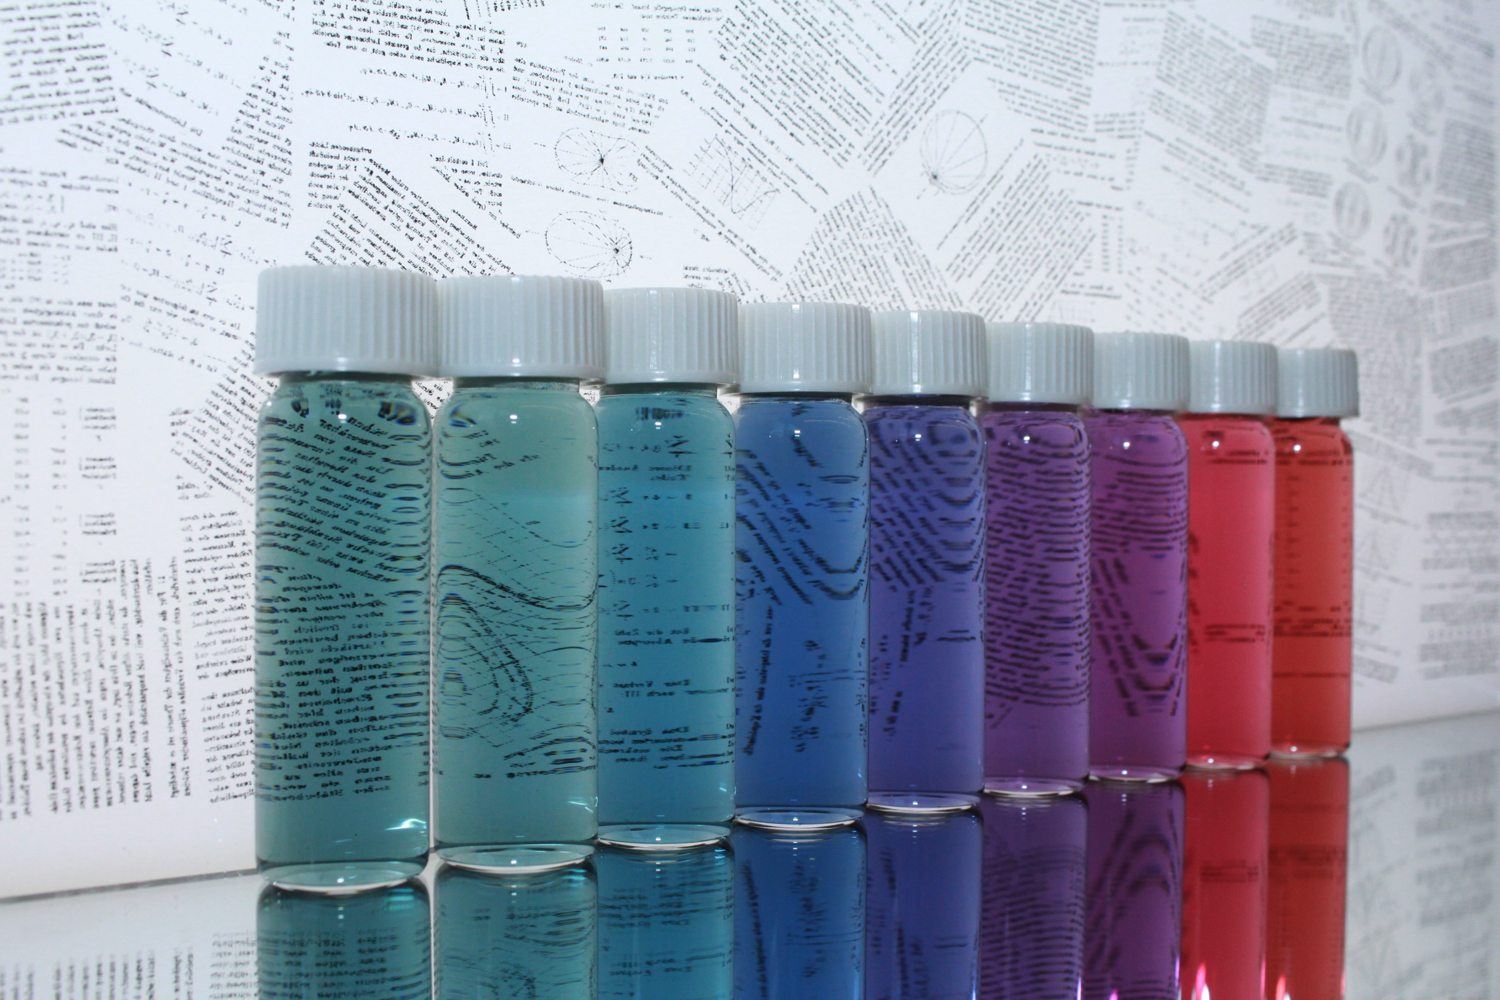
\includegraphics[width=150mm,scale=1.5]{Untitled.png}
\end{figure}
\clearpage
\end{center} 
% END TITLE
%\maketitle
\newgeometry{margin=3cm}
\thispagestyle{empty}
%\begin{abstract}
\vspace*{2cm}
\begin{center} 
{\Large ABSTRACT}\par
\end{center} 
\vspace*{1cm}
\noindent
Lateral flow devices are ideal candidates for diagnosis of disease in remote areas, due to their low cost and rapid readout. Moreover, they can be stored at relatively high temperatures, and do not require electric power, specialized personnel, equipment or reagents. We planned to use those devices to diagnose dengue, a tropical disease that has caused major epidemics and hospitalization in the last decades. It was observed during the last ebola outbreak that because of the large amount of patients, medical decisions (such as quarantine) were often made based on the symptoms of patients, instead of diagnostic data. The initial symptoms of ebola are similar to dengue and other viral illnesses, which caused numerous patients to be mistakenly quarantined with ebola patients, and putting their lives in danger. The reason for that was the non-existence of an ebola rapid diagnostic. As a response, we have recently included ebola, zika and chikungunya in our original dengue panel test.\\ 
Lateral flow devices use capillary flow and the accumulation of ligand-coated gold nanoparticles to detect the presence of target proteins. Unfortunately, an issue of lateral flow devices is their low sensitivity and specificity, which greatly depends on the nature of the ligand-target pair and their binding thermodynamics on the surface. The focus of this report will be on the diagnosis of tropical viral infections, namely: dengue, chikungunya, zika and ebola. Moreover, we will focus on the improvement of lateral flow devices by tuning the physical and chemical properties of the gold nanoparticles that give the colorimetric readout. Also, we tune the physical and chemical properties of the paperfluidic strip, in order to improve the sensitivity of the devices. \\
These new, effective, fast, reliable and inexpensive lateral flow devices will represent significant improvements to field detection of disease in situations where there is a lack of specialized personnel, reagents or materials challenge the suitability of the standard diagnosis methods. By allowing mobile phone readability of the diagnosis results, we will be able to obtain real-time epidemiologic data on the spread of the disease.\\
\vspace*{1cm}


\begin{minipage}[t]{5cm}
\flushleft
\noindent
Ph.D. Advisor:\\
Prof. Lee Gehrke\\
+1 617 253 7608\\
lgehrke@mit.edu\\
\href{http://www.gehrkelab.org}{gehrkelab.org}
\end{minipage}
\hfill
\begin{minipage}[t]{5cm}
\flushright
\null
Helena de Puig \\+1 617 599 3390\\hpuig@mit.edu\\\href{http://www.hpuig.mit.edu}{hpuig.mit.edu}
\end{minipage}
\vfill
\noindent
\textbf{Keywords:} nanoparticle, dengue, zika, chikungunya, ebola, tropical viruses, lateral flow immunoassays, diagnostics, rapid test, paperfluidic, infectious diseases, nanoparticles, real-time epidemiology, mobile phone technologies, aedes aegypti, aedes albopictus
%\end{abstract}
\restoregeometry
\newpage
\section{Introduction}
Viral hemorrhagic fever viruses require special attention for public health preparedness due to their transmissibility and cause of high mortality1, 2.  In particular, dengue is transmitted by the mosquitos Aedes aegypti and Aedes albopictus, and is a major international health concern because its dissemination has increased greatly in urban areas due to travel and globalization3. The WHO estimates that there are 50-100 million infections yearly, and 2.5 billion people at risk of dengue. There are four distinct viral serotypes (DEN 1-4). Recovery from infection by one provides lifelong immunity against that particular serotype, but subsequent infections by other serotypes increase the risk of developing dengue hemorrhagic fever (DHF) or dengue shock syndrome (DSS)4. \\
Accurate diagnosis of dengue fever is critical to treat individual patients and to predict the potential of epidemics resulting from the introduction of a dengue serotype previously unknown to an area5. The current methods for dengue detection include thermal cycling amplification (PCR)6 and enzyme-linked immunoabsorbent assays (ELISA)7. However, these methods require specialized equipment, reagents, and highly trained personnel, have a complex methodology, and a slow turnaround for readout, challenging their suitability in the field8. Immunochromatography assays, also known as lateral flow tests, on the other hand, are simple, easy to use, low-cost diagnostic tools that provide fast detection of antibodies or antigens9, 10. \\
Lateral flow is an ideal method for detecting disease in remote areas because the need for refrigerated storage can be obviated; moreover, specialized chemicals and expertise are not needed11. Lateral flow tests (Figure 1) use capillary action to move sample conjugates and reagents through a porous nitrocellulose membrane11, 12. The conjugate pad contains the detection conjugate, which can be any species that gives rise to a color13. Typically this is spherical gold nanoparticles bound to an antibody or biomolecule that can specifically capture the test protein. Once the test solution is placed on the sample pad, it flows toward the conjugate pad and mixes with the detection conjugate. It then flows to the absorbent pad, passing through the nitrocellulose membrane, where the detection antibodies have been printed an antibody against the agent to be detected in the test line, a positive control and negative control. A visible line can be observed when gold nanoparticles accumulate in a specific region due to ligand-receptor binding. Therefore, if the test protein is present in the test solution, the gold nanoparticles will accumulate at both the positive control and test lines. Lateral flow strips are widely used in point of care (POC) devices, such as pregnancy tests, disease diagnostics, etc. because they can be operated by non-experts, they are cheap, portable, and do not require electric power to be operated10. \\
The central element of lateral flow devices is the gold nanoparticles that give rise to the colorimetric readout. The strong absorption of light by gold nanoparticles is due to the electron oscillations on their surface, which depends on the size and shape of the nanoparticles15. Therefore, it is possible to design gold nanoparticles to have high absorption even at low concentrations. Spherical gold nanoparticles show a surface plasmon resonance peak at a wavelength of around 520nm. In the case of gold nanorods, their unique properties rely on their lack of symmetry16. When the nanoparticles are elongated in one of their dimensions it is possible to observe a secondary peak at higher wavelengths, called longitudinal surface plasmon resonance (LSPR)17. Therefore, short nanorods show two absorption peaks (one around 550nm, and a second one at 650nm), and long nanorods show absorption peaks at 800nm and 520nm. It is possible to maximize nanoparticle absorption in the range where the human eye can see –between 390 and 700nm-, and/or the spectral detection range of a typical mobile phone camera, and therefore increase the visibility of the test band in the lateral flow device, even at low concentrations. In order to do that, we have synthesized gold nanoparticles with different sizes and shapes –nanorods18-20, nanospheres21-23 and nanostars24-, and tested them for increased sensitivity in lateral flow devices. \\
Here, we build machine-readable multiplexed lateral flow devices for the detection of 8-10 tropical disease markers. By making them so that a mobile phone can read them, the device will be able to provide real-time epidemiologic data to monitor disease distribution based on diagnostic data (Figure 1). Gold nanoparticle conjugates and the antibodies used to detect the disease biomarkers are critical to ensure that the devices have enough sensitivity to detect the illness even at low concentrations of target protein, such as in early stages of the disease. By optimizing the properties of the device it is possible to lower its cost, as it would enable to lower the amount of antibodies and nanoparticles used in the device. My thesis project consists in engineering the nanoparticle material properties, their surface chemistry, and biofunctionalization to increase the sensitivity of lateral flow detection. \\

\newpage
\section{Research Approach and Methods}

\section{Results}

Comments can be added to your project by clicking on the comment icon in the toolbar above. % * <john.hammersley@gmail.com> 2014-09-03T09:54:16.211Z:
%
% Here's an example comment!
%
To reply to a comment, simply click the reply button in the lower right corner of the comment, and you can close them when you're done.

\subsection{How to include Figures}

First you have to upload the image file from your computer using the upload link the project menu. Then use the includegraphics command to include it in your document. Use the figure environment and the caption command to add a number and a caption to your figure. See the code for Figure \ref{fig:frog} in this section for an example.

\begin{figure}
\centering
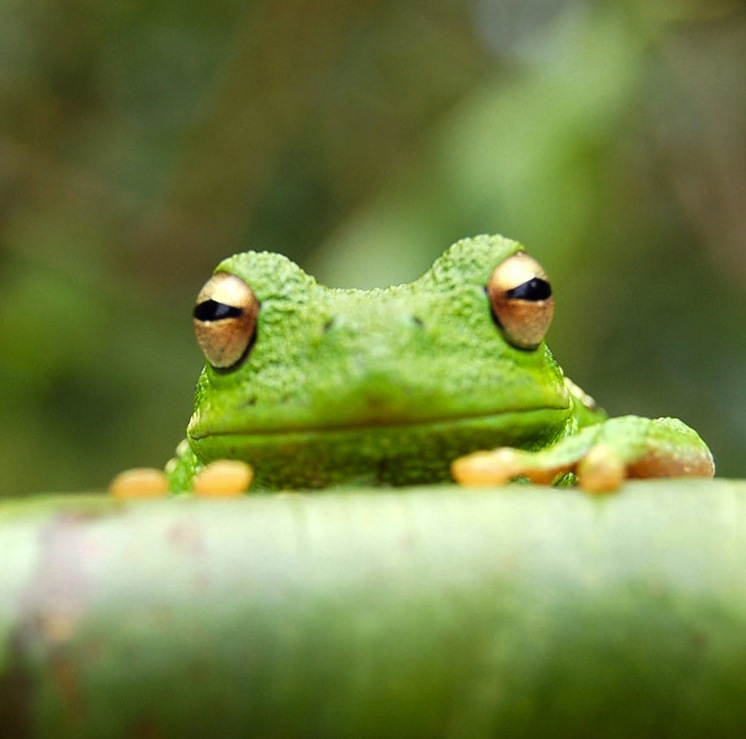
\includegraphics[width=0.3\textwidth]{frog.jpg}
\caption{\label{fig:frog}This frog was uploaded via the project menu.}
\end{figure}

\subsection{How to add Tables}

Use the table and tabular commands for basic tables --- see Table~\ref{tab:widgets}, for example. 

\begin{table}
\centering
\begin{tabular}{l|r}
Item & Quantity \\\hline
Widgets & 42 \\
Gadgets & 13
\end{tabular}
\caption{\label{tab:widgets}An example table.}
\end{table}

\subsection{How to write Mathematics}

\LaTeX{} is great at typesetting mathematics. Let $X_1, X_2, \ldots, X_n$ be a sequence of independent and identically distributed random variables with $\text{E}[X_i] = \mu$ and $\text{Var}[X_i] = \sigma^2 < \infty$, and let
$$S_n = \frac{X_1 + X_2 + \cdots + X_n}{n}
      = \frac{1}{n}\sum_{i}^{n} X_i$$
denote their mean. Then as $n$ approaches infinity, the random variables $\sqrt{n}(S_n - \mu)$ converge in distribution to a normal $\mathcal{N}(0, \sigma^2)$.


\subsection{How to create Sections and Subsections}

Use section and subsections to organize your document. Simply use the section and subsection buttons in the toolbar to create them, and we'll handle all the formatting and numbering automatically.

\subsection{How to add Lists}

You can make lists with automatic numbering \dots

\begin{enumerate}
\item Like this,
\item and like this.
\end{enumerate}
\dots or bullet points \dots
\begin{itemize}
\item Like this,
\item and like this.
\end{itemize}

We hope you find Overleaf useful, and please let us know if you have any feedback using the help menu above.

\end{document}